\subsection{Proportion of Age}
Our first aim was to have an overall understanding of the mothers' age group and their proportions. After performing some statistical analysis we get two figures that show the trends of mothers of different age groups and their habits when it comes to having babies. In Figure: \ref{fig:age1} we can see that the age group of 15-19 and over 40 are the last 2 age groups that have babies while most mothers are from the age group of 30-34. 

\begin{figure}
  \centering
  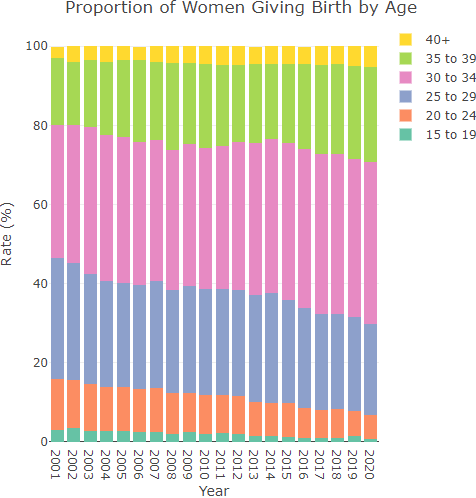
\includegraphics[width=0.35\textwidth]{img/age_group.png}
  \caption{Proportion of woman giving birth by age.}
  \label{fig:age1}
\end{figure}